\documentclass[11pt]{texMemo-gibbons}
\usepackage[english]{babel}
\usepackage{graphicx}
\usepackage{blindtext}
\usepackage{amsmath,amssymb,units}
\usepackage{siunitx}
\usepackage[outdir=./]{epstopdf}
\usepackage{subfigure}
\memostudent{Ty Davis}
\memocourse{ECE 3210}
\memosubject{Lab 8, Designing a Low-pass Filter}
\memodate{\today}
\logo{
\includegraphics[width=0.5\textwidth]{ece_horiz.pdf}}

\begin{document}
\maketitle

\section{Introduction}
\label{sec:introduction}

In this lab we are building a 2nd order Sallen-Key low
pass filter. We will have to select the component avlues
ourselves, after which we will build the circuit and
compare the results.

\section{Theory}
\label{sec:theory}

Fig.~\ref{fig:circuit} shows the circuit that we are 
using. To select the values of the components,
we need to derive a transfer function for the circuit.

We can analyze this circuit with two nodal-analyses,
which are shown as follows:

\[
  \frac{V_s - V_i}{R_1} + \frac{V_s - V_0}{R_2} + \frac{V_s - V_0}{1/(sC_1)} = 0
\]

\[
  \frac{V_0}{1/(sC_2)} + \frac{V_0 - V_s}{R_2} = 0
\]

Rearranging these two expressions and combining them 
we get the tranfer function, shown in Eq.~\ref{eq:transfer}.

\begin{equation}
  H(s) = \frac{1 / (R_1 R_2 C_1 C_2)}{s^2 + s \frac{R_1 + R_2}{ R_1 R_2 C_1} + \frac{1}{R_1 R_2 C_1 C_2}}
  \label{eq:transfer}
\end{equation}

This can be mapped to the Sallen-Key transfer function if we used the following
equations:

\[
  \omega_c = \frac{1}{\sqrt{R_1 R_2 C_1 C_2}}
\]

\[
  \zeta = \frac{1}{R_1 C_1} + \frac{1}{R_2 C_1}
\]

To build the circuit with a cutoff frequency of 10~kHz
and a damping ratio of 0.5 (underdamped), we were able
to select values for the resistors and capacitors. We
chose $R_1 = 220~\si\ohm$, and $R_2 = 220~\si\ohm$,
and accordingly calculated $C_1 = 144.7~\si\nF$, and
$C_2 = 36.17~\si\nF$.



\section{Results}
\label{sec:results}

Building the circuit we used $C_1 = 150~\si\nF$ and
$C_2 = 33~\si\nF$. These values were close enough to 
the calculated values and proved effective for the circuit.

The three Figs.~\ref{fig:calc}, \ref{fig:sim}, and \ref{fig:meas}
show the frequency response of the circuit when calculated,
simulated, and measured. The plots show similar patterns,
note the bump at the knee of the gain curve, as well
as the slope of the gain curve after the cutoff frequency.

\section{Discussion and Conclusions}
\label{sec:conclusions}

The simulation and measurements both show that the components
that we selected created an effective filter. Right at 10~kHz
the gain starts to drop significantly, it shows as a rate of
about 20~dB per decade. The bump before the cutoff frequency
occurs because the circuit is underdamped, just as we designed
the circuit for with those components.


\clearpage

\begin{figure}
  \begin{center}
    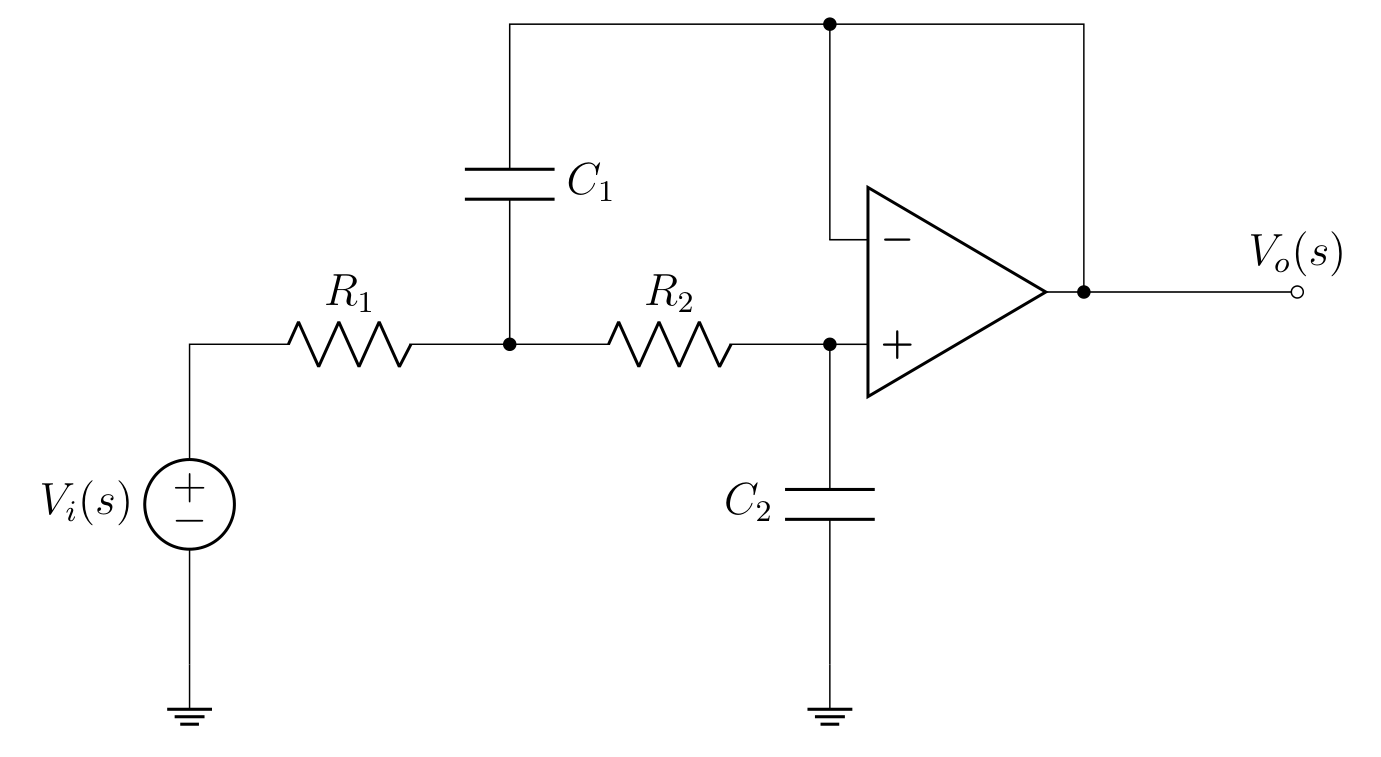
\includegraphics[width=0.75\textwidth]{../figures/circuit.png}
  \end{center}
  \caption{Sallen-Key Circuit}\label{fig:circuit}
\end{figure}

\begin{figure}
  \begin{center}
    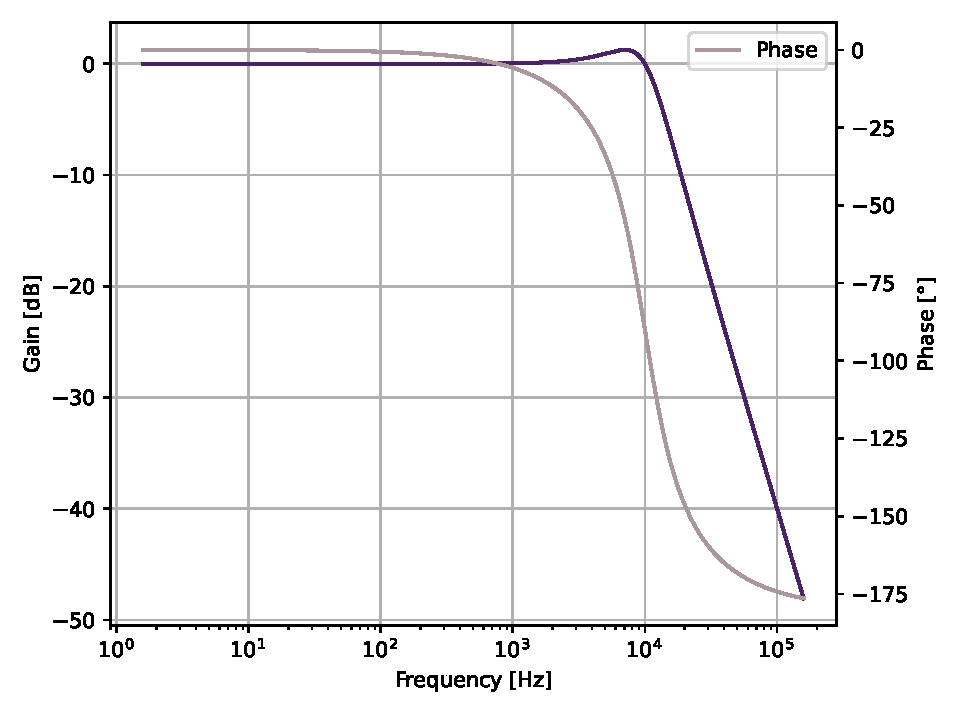
\includegraphics[width=0.75\textwidth]{../pdf/calculation.pdf}
  \end{center}
  \caption{Calculation Results}\label{fig:calc}
\end{figure}

\begin{figure}
  \begin{center}
    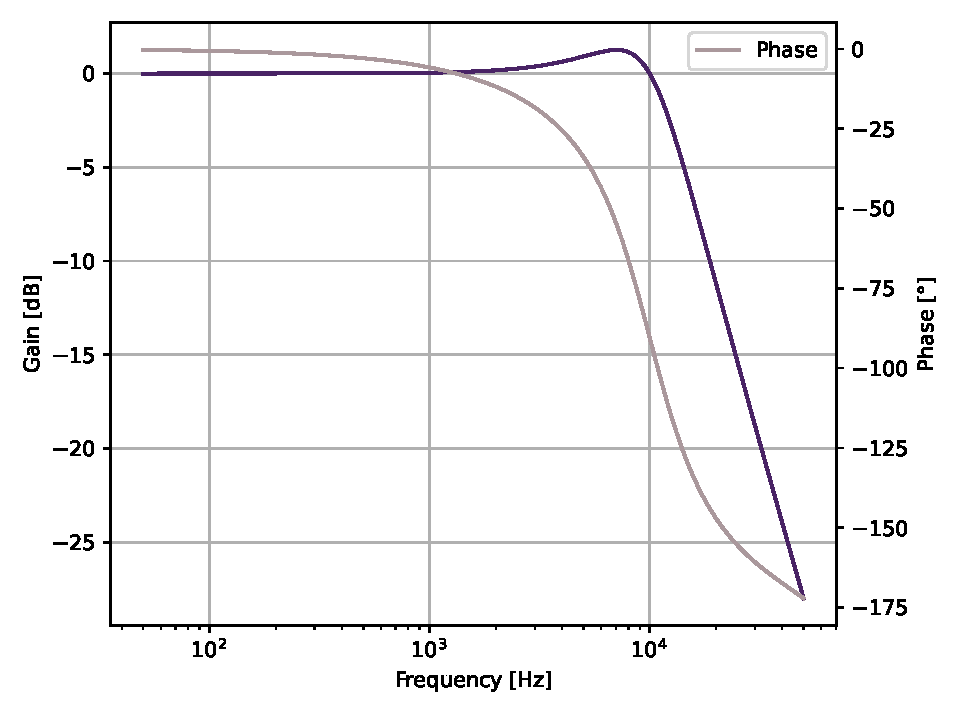
\includegraphics[width=0.75\textwidth]{../pdf/simulation.pdf}
  \end{center}
  \caption{Simulation Results}\label{fig:sim}
\end{figure}

\begin{figure}
  \begin{center}
    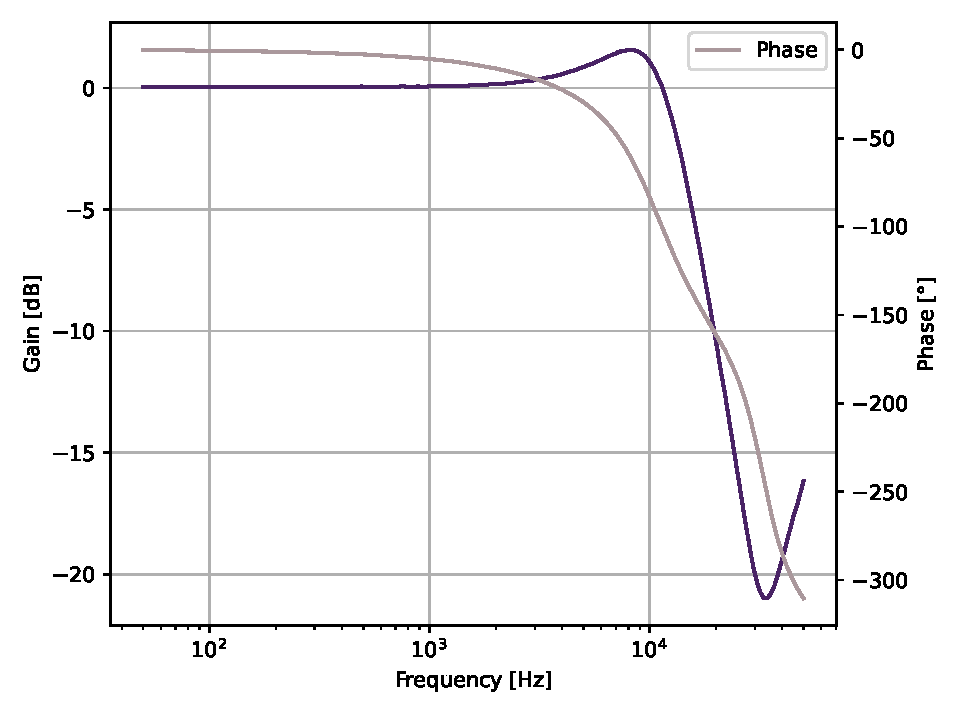
\includegraphics[width=0.75\textwidth]{../pdf/measurements.pdf}
  \end{center}
  \caption{Measurement Results}\label{fig:meas}
\end{figure}


\end{document}
